% !TeX encoding = UTF-8
% !TeX program = xelatex
% !TeX spellcheck = en_US

\documentclass[degree=master]{thuthesis}
  % 学位 degree:
  %   doctor | master | bachelor | postdoc
  % 学位类型 degree-type:
  %   academic(默认)| professional
  % 语言 language
  %   chinese(默认)| english
  % 字体库 fontset
  %   windows | mac | fandol | ubuntu
  % 建议终版使用 Windows 平台的字体编译


% 论文基本配置,加载宏包等全局配置
% !TeX root = ./thuthesis-example.tex

% 论文基本信息配置

\thusetup{
  %******************************
  % 注意:
  %   1. 配置里面不要出现空行
  %   2. 不需要的配置信息可以删除
  %   3. 建议先阅读文档中所有关于选项的说明
  %******************************
  %
  % 输出格式
  %   选择打印版(print)或用于提交的电子版(electronic),前者会插入空白页以便直接双面打印
  %
  output = print,
  % 格式类型
  %   默认为论文(thesis),也可以设置为开题报告(proposal)
  % thesis-type = proposal,
  %
  % 标题
  %   可使用“\\”命令手动控制换行
  %
  title  = {量子线路的观测值模拟},
  title* = {Simulating observables of quantum circuits},
  %
  % 学科门类
  %   1. 学术型
  %      - 中文
  %        需注明所属的学科门类,例如:
  %        哲学、经济学、法学、教育学、文学、历史学、理学、工学、农学、医学、
  %        军事学、管理学、艺术学
  %      - 英文
  %        博士:Doctor of Philosophy
  %        硕士:
  %          哲学、文学、历史学、法学、教育学、艺术学门类,公共管理学科
  %          填写“Master of Arts“,其它填写“Master of Science”
  %   2. 专业型
  %      直接填写专业学位的名称,例如:
  %      教育博士、工程硕士等
  %      Doctor of Education, Master of Engineering
  %   3. 本科生不需要填写
  %
  degree-category  = {理学博士},
  degree-category* = {Doctor of Philosophy},
  %
  % 培养单位
  %   填写所属院系的全名
  %
  department = {数学科学系},
  %
  % 学科
  %   1. 研究生学术型学位,获得一级学科授权的学科填写一级学科名称,其他填写二级学科名称
  %   2. 本科生填写专业名称,第二学位论文需标注“(第二学位)”
  %
  discipline  = {数学},
  discipline* = {Mathmathics},
  %
  % 专业领域
  %   1. 设置专业领域的专业学位类别,填写相应专业领域名称
  %   2. 2019 级及之前工程硕士学位论文,在 `engineering-field` 填写相应工程领域名称
  %   3. 其他专业学位类别的学位论文无需此信息
  %
  % professional-field  = {计算机技术},
  % professional-field* = {Computer Technology},
  %
  % 姓名
  %
  author  = {邵钰菓},
  author* = {Yuguo Shao},
  %
  % 学号
  % 仅当书写开题报告时需要(同时设置 `thesis-type = proposal')
  %
  % student-id = {2000310000},
  %
  % 指导教师
  %   中文姓名和职称之间以英文逗号“,”分开,下同
  %
  supervisor  = {刘正伟, 教授},
  supervisor* = {Professor Zhengwei Liu},
  %
  % 副指导教师
  %
  %associate-supervisor  = {陈文光, 教授},
  %associate-supervisor* = {Professor Chen Wenguang},
  %
  % 联合指导教师
  %
  % co-supervisor  = {某某某, 教授},
  % co-supervisor* = {Professor Mou Moumou},
  %
  % 日期
  %   使用 ISO 格式;默认为当前时间
  %
  % date = {2019-07-07},
  %
  % 是否在中文封面后的空白页生成书脊(默认 false)
  %
  include-spine = false,
  %
  % 密级和年限
  %   秘密, 机密, 绝密
  %
  % secret-level = {秘密},
  % secret-year  = {10},
  %
  % 博士后专有部分
  %
  % clc                = {分类号},
  % udc                = {UDC},
  % id                 = {编号},
  % discipline-level-1 = {计算机科学与技术},  % 流动站(一级学科)名称
  % discipline-level-2 = {系统结构},          % 专业(二级学科)名称
  % start-date         = {2011-07-01},        % 研究工作起始时间
}

% 载入所需的宏包

% 定理类环境宏包
\usepackage{amsthm}
% 也可以使用 ntheorem
% \usepackage[amsmath,thmmarks,hyperref]{ntheorem}

\thusetup{
  %
  % 数学字体
  % math-style = GB,  % GB | ISO | TeX
  math-font  = xits,  % stix | xits | libertinus
}

% 可以使用 nomencl 生成符号和缩略语说明
% \usepackage{nomencl}
% \makenomenclature

% 表格加脚注
\usepackage{threeparttable}

% 表格中支持跨行
\usepackage{multirow}
\usepackage{physics}
% 固定宽度的表格。
% \usepackage{tabularx}

% 跨页表格
\usepackage{longtable}

% 算法
\usepackage{algorithm}
\usepackage{algorithmic}

% 量和单位
\usepackage{siunitx}
\usepackage{quantikz}

% 参考文献使用 BibTeX + natbib 宏包
% 顺序编码制
\usepackage[sort]{natbib}
\bibliographystyle{thuthesis-numeric}

% 著者-出版年制
% \usepackage{natbib}
% \bibliographystyle{thuthesis-author-year}

% 生命科学学院要求使用 Cell 参考文献格式(2023 年以前使用 author-date 格式)
% \usepackage{natbib}
% \bibliographystyle{cell}

% 本科生参考文献的著录格式
% \usepackage[sort]{natbib}
% \bibliographystyle{thuthesis-bachelor}

% 参考文献使用 BibLaTeX 宏包
% \usepackage[style=thuthesis-numeric]{biblatex}
% \usepackage[style=thuthesis-author-year]{biblatex}
% \usepackage[style=gb7714-2015]{biblatex}
% \usepackage[style=apa]{biblatex}
% \usepackage[style=mla-new]{biblatex}
% 声明 BibLaTeX 的数据库
% \addbibresource{ref/refs.bib}

% 定义所有的图片文件在 figures 子目录下
\graphicspath{{figures/}}

% 数学命令
\makeatletter
\newcommand\dif{%  % 微分符号
  \mathop{}\!%
  \ifthu@math@style@TeX
    d%
  \else
    \mathrm{d}%
  \fi
}
\makeatother

% hyperref 宏包在最后调用
\usepackage{hyperref}

\newcommand{\supp}{\text{supp}}
\newcommand{\poly}{\text{Poly}}


\begin{document}

% 封面
\maketitle

% 学位论文指导小组、公开评阅人和答辩委员会名单
% 本科生不需要
% !TeX root = ../thuthesis-example.tex

%\begin{committee}[name={学位论文指导小组、公开评阅人和答辩委员会名单}]
\begin{committee}[name={学位论文公开评阅人和答辩委员会名单}]
  \newcolumntype{C}[1]{@{}>{\centering\arraybackslash}p{#1}}

  \section*{指导小组名单}

  \begin{center}
    \begin{tabular}{C{3cm}C{3cm}C{9cm}@{}}
      刘正伟 & 教授     & 清华大学 
  %    王XX & 副教授   & 清华大学 \\
  %    张XX & 助理教授 & 清华大学 \\
    \end{tabular}
  \end{center}


  \section*{公开评阅人名单}

  \begin{center}
    \begin{tabular}{C{3cm}C{3cm}C{9cm}@{}}
      骆顺龙	& 研究员   & 中国科学院数学与系统科学研究院\\
      魏朝晖 & 助理教授 & 清华大学\\
      张潘 & 研究员 & 中国科学院理论物理研究所 \\
      袁骁 & 助理教授 & 北京大学 
    \end{tabular}
  \end{center}


  \section*{答辩委员会名单}

  \begin{center}
    \begin{tabular}{C{2.75cm}C{2.98cm}C{4.63cm}C{4.63cm}@{}}
      主席 & 郑浩                  & 教授                    & 清华大学       \\
      委员 & 肖杰                  & 教授                    & 北京师范大学       \\
         & \multirow{2}{*}{骆顺龙} & \multirow{2}{*}{研究员} & 中国科学院 \\
         &                       &                         & 数学与系统科学研究院  \\
        %& 骆顺龙                  & 研究员                    & 中国科学院数学与系统科学研究院       \\
          & 左怀青                  & 教授                  & 清华大学       \\
          & 魏朝晖                  & 助理教授                  & 清华大学       \\
      秘书 & 李慧慧                  & 博士后              & 清华大学       \\
    \end{tabular}
  \end{center}
\end{committee}



% 也可以导入 Word 版转的 PDF 文件
% \begin{committee}[file=figures/committee.pdf]
% \end{committee}


% 使用授权的说明
% 本科生开题报告不需要
\copyrightpage
% 将签字扫描后授权文件 scan-copyright.pdf 替换原始页面
% \copyrightpage[file=scan-copyright.pdf]

\frontmatter
% !TeX root = ../thuthesis-example.tex

% 中英文摘要和关键字

\begin{abstract}
  量子计算的经典模拟是验证量子硬件、优化算法设计及探索量子优势边界的重要工具。本文针对含噪声中等规模量子(NISQ)设备的模拟需求,提出基于Pauli路径积分的高效经典模拟方法,系统分析其计算复杂度与误差特性,并验证其实际应用价值。

  大规模变分量子算法被广泛认为是实现实用量子优势的潜在途径。然而,量子噪声的存在可能会抑制并削弱这些优势,这使得经典可模拟性的界限变得模糊。为了进一步澄清这一问题,我们提出了一种基于可观测量在泡利路径上反向传播路径积分(OBPPP)的新型多项式规模方法。该方法能够在单量子比特泡利噪声存在的情况下,以有界截断误差高效近似变分量子算法中算子的期望值。理论上我们严格证明:1)当最小非零噪声率γ为常数时,OBPPP的时间与空间复杂度与量子比特数n、电路深度L呈现多项式关系;2)对于可变的γ,当存在超过两个非零噪声因子时,若γ大于1/log L则复杂度保持Poly(n, L),但若γ低于1/L时复杂度将随L呈指数增长。数值方面,我们对IBM在127量子比特鹰处理器上进行的零噪声外推实验结果[Nature 618, 500 (2023)]进行了经典模拟。相比量子设备,我们的方法获得了更高的精度与更快的运行速度。此外,我们的方法能够模拟含噪声结果,精确复现了IBM未经误差缓解、与原始实验观测直接对应的计算结果。本研究表明噪声在经典模拟中的关键作用,所提出的方法适用于广泛量子电路的期望值计算,在量子计算机验证领域具有普适性。



  论文的摘要是对论文研究内容和成果的高度概括。
  摘要应对论文所研究的问题及其研究目的进行描述,对研究方法和过程进行简单介绍,对研究成果和所得结论进行概括。
  摘要应具有独立性和自明性,其内容应包含与论文全文同等量的主要信息。
  使读者即使不阅读全文,通过摘要就能了解论文的总体内容和主要成果。

  论文摘要的书写应力求精确、简明。
  切忌写成对论文书写内容进行提要的形式,尤其要避免“第 1 章……;第 2 章……;……”这种或类似的陈述方式。

  关键词是为了文献标引工作、用以表示全文主要内容信息的单词或术语。
  关键词不超过 5 个,每个关键词中间用分号分隔。

  % 关键词用“英文逗号”分隔,输出时会自动处理为正确的分隔符
  \thusetup{
    keywords = {量子计算, 量子线路经典模拟 , Pauli路径积分, 变分量子算法, 量子噪声},
  }
\end{abstract}

\begin{abstract*}
  An abstract of a dissertation is a summary and extraction of research work and contributions.
  Included in an abstract should be description of research topic and research objective, brief introduction to methodology and research process, and summary of conclusion and contributions of the research.
  An abstract should be characterized by independence and clarity and carry identical information with the dissertation.
  It should be such that the general idea and major contributions of the dissertation are conveyed without reading the dissertation.

  An abstract should be concise and to the point.
  It is a misunderstanding to make an abstract an outline of the dissertation and words “the first chapter”, “the second chapter” and the like should be avoided in the abstract.

  Keywords are terms used in a dissertation for indexing, reflecting core information of the dissertation.
  An abstract may contain a maximum of 5 keywords, with semi-colons used in between to separate one another.

  % Use comma as separator when inputting
  \thusetup{
    keywords* = {keyword 1, keyword 2, keyword 3, keyword 4, keyword 5},
  }
\end{abstract*}


% 目录
\tableofcontents

% 插图和附表清单
% 本科生的插图索引和表格索引需要移至正文之后、参考文献前
% \listoffiguresandtables  % 插图和附表清单(仅限研究生)
\listoffigures           % 插图清单
\listoftables            % 附表清单

% 符号对照表
% !TeX root = ../thuthesis-example.tex

\begin{denotation}[3cm]
  \item[CPD] Clifford数据回归(Clifford Data Regression)
  \item[CPDR] Clifford扰动数据回归(Clifford Perturbation Data Regression)
  \item[CPTP] 完全正保迹(Completely Positive and Trace-Preserving) 
  \item[DMRG] 密度矩阵重整化群(Density Matrix Renormalization Group)
  \item[MPS] 矩阵乘积态(Matrix Product State) 
  \item[MSE] 均方误差(Mean Squared Error) 
  \item[NISQ] 含噪声中等规模量子(Noisy Intermediate-Scale Quantum)
  \item[OBPPP] 可观测量在Pauli路径下的反向传播算法(Observable's Back-Propagation on Pauli Path)
  \item[POVM] 正算子值测量(Positive Operator-Valued Measure)
  \item[QAOA] 量子近似优化算法(Quantum Approximate Optimization Algorithm)
  \item[QEC] 量子纠错(Quantum Error Correction)
  \item[Qubit] 量子比特(Quantum Bit)
  \item[QSVM] 量子支持向量机(Quantum Support Vector Machine) 
  \item[QNN] 量子神经网络(Quantum Neural Network) 
  \item[RRMSE] 相对均方根误差(Relative Root Mean Square Error) 
  \item[SPD] 稀疏Pauli动力学 (Sparse Pauli Dynamics)
  \item[SVD] 奇异值分解(Singular Value Decomposition)
  \item[VQA] 变分量子算法(Variational Quantum Algorithm) 
  \item[VQE] 变分量子本征求解器(Variational Quantum Eigensolver)
  \item[ZNE] 零噪声推断(Zero-Noise Extrapolation)
  
  
\end{denotation}



% 也可以使用 nomencl 宏包,需要在导言区
% \usepackage{nomencl}
% \makenomenclature

% 在这里输出符号说明
% \printnomenclature[3cm]

% 在正文中的任意为都可以标题
% \nomenclature{PI}{聚酰亚胺}
% \nomenclature{MPI}{聚酰亚胺模型化合物,N-苯基邻苯酰亚胺}
% \nomenclature{PBI}{聚苯并咪唑}
% \nomenclature{MPBI}{聚苯并咪唑模型化合物,N-苯基苯并咪唑}
% \nomenclature{PY}{聚吡咙}
% \nomenclature{PMDA-BDA}{均苯四酸二酐与联苯四胺合成的聚吡咙薄膜}
% \nomenclature{MPY}{聚吡咙模型化合物}
% \nomenclature{As-PPT}{聚苯基不对称三嗪}
% \nomenclature{MAsPPT}{聚苯基不对称三嗪单模型化合物,3,5,6-三苯基-1,2,4-三嗪}
% \nomenclature{DMAsPPT}{聚苯基不对称三嗪双模型化合物(水解实验模型化合物)}
% \nomenclature{S-PPT}{聚苯基对称三嗪}
% \nomenclature{MSPPT}{聚苯基对称三嗪模型化合物,2,4,6-三苯基-1,3,5-三嗪}
% \nomenclature{PPQ}{聚苯基喹噁啉}
% \nomenclature{MPPQ}{聚苯基喹噁啉模型化合物,3,4-二苯基苯并二嗪}
% \nomenclature{HMPI}{聚酰亚胺模型化合物的质子化产物}
% \nomenclature{HMPY}{聚吡咙模型化合物的质子化产物}
% \nomenclature{HMPBI}{聚苯并咪唑模型化合物的质子化产物}
% \nomenclature{HMAsPPT}{聚苯基不对称三嗪模型化合物的质子化产物}
% \nomenclature{HMSPPT}{聚苯基对称三嗪模型化合物的质子化产物}
% \nomenclature{HMPPQ}{聚苯基喹噁啉模型化合物的质子化产物}
% \nomenclature{PDT}{热分解温度}
% \nomenclature{HPLC}{高效液相色谱(High Performance Liquid Chromatography)}
% \nomenclature{HPCE}{高效毛细管电泳色谱(High Performance Capillary lectrophoresis)}
% \nomenclature{LC-MS}{液相色谱-质谱联用(Liquid chromatography-Mass Spectrum)}
% \nomenclature{TIC}{总离子浓度(Total Ion Content)}
% \nomenclature{\textit{ab initio}}{基于第一原理的量子化学计算方法,常称从头算法}
% \nomenclature{DFT}{密度泛函理论(Density Functional Theory)}
% \nomenclature{$E_a$}{化学反应的活化能(Activation Energy)}
% \nomenclature{ZPE}{零点振动能(Zero Vibration Energy)}
% \nomenclature{PES}{势能面(Potential Energy Surface)}
% \nomenclature{TS}{过渡态(Transition State)}
% \nomenclature{TST}{过渡态理论(Transition State Theory)}
% \nomenclature{$\increment G^\neq$}{活化自由能(Activation Free Energy)}
% \nomenclature{$\kappa$}{传输系数(Transmission Coefficient)}
% \nomenclature{IRC}{内禀反应坐标(Intrinsic Reaction Coordinates)}
% \nomenclature{$\nu_i$}{虚频(Imaginary Frequency)}
% \nomenclature{ONIOM}{分层算法(Our own N-layered Integrated molecular Orbital and molecular Mechanics)}
% \nomenclature{SCF}{自洽场(Self-Consistent Field)}
% \nomenclature{SCRF}{自洽反应场(Self-Consistent Reaction Field)}



% 正文部分
\mainmatter
\chapter{绪论}

\section{研究背景}

量子力学的建立和发展是20世纪人类科学领域最伟大的科学突破之一,它不仅解决了经典物理学在描述微观世界中的失败,而且在许多方面都超越了经典物理学。量子力学的建立不仅推动了物理学的发展,而且对其他学科的发展也产生了深远的影响,许多新兴的领域和学科就此产生,如量子信息科学。

量子信息科学是量子力学和信息科学的交叉领域,它主要研究如何利用量子力学的特性来处理和传输信息。在当今信息时代,信息的处理和传输已经成为人们生活中不可或缺的一部分。
自1940年代,第一台电子计算机诞生以来,计算机技术已经取得了长足的进步,计算机的性能也在不断提高。
英特尔公司创始人戈登·摩尔在1965年提出的摩尔定律,预言单个集成电路上可容纳的晶体管数目每隔18个到24个月就会翻一番。
这一定律不是一个自然定律,而是人们在经验上总结出来的一个规律,但是在过去的几十年中,摩尔定律一直被证明是正确的。但是随着计算机技术的不断发展,集成电路的尺寸越来越小,逐渐接近原子尺度。
在原子尺度下,经典物理学的规律不再适用,量子效应开始显现,这就导致了集成电路的性能难以继续提高,摩尔定律也逐渐失效。

而随着人工智能、大数据、物联网等新兴技术的发展,对计算机性能的需求也越来越高。在这种情况下,传统的计算机技术已经无法满足人们的需求,因此人们开始寻找新的计算机技术。量子计算机作为一种新型的计算机技术,具有很大的发展潜力,并被认为是未来计算机技术的发展方向之一。

在1980年代,Benioff、Manin、Feynman等人提出了量子计算机的概念~\cite{Benioff1980,Benioff1982a,Benioff1982b,Manin1980,Feynman1982}。
最初的动机是希望利用量子力学的特性来模拟量子系统,如果使用经典计算机来模拟量子系统,需要耗费大量的计算资源,而量子计算机可以更加高效地模拟量子系统。后来的研究表明,量子计算机不仅可以模拟量子系统,而且可以解决一些经典计算机难以处理的问题。
1994年,Shor提出了一种基于量子计算机的大整数分解算法~\cite{shor1994algorithms},该算法可以在多项式时间内分解大整数,这对于现代密码学体系具有重要意义。
时至今日,量子计算的研究吸引了众多科学家的关注,也在各个领域衍生出了广泛的应用,包括密码学、量子化学~\cite{peruzzo2014variational, Kandala2017hardware,li2022toward}、量子机器学习~\cite{beer2020training,huang2021experimental,havlivcek2019supervised,mitarai2018quantum}、量子优化算法~\cite{farhi2014quantum,moll2018quantum}等。
此外,除了量子计算之外,量子信息还包括量子纠错、量子复杂度、量子通信、量子传感、量子控制等领域,这些领域也为量子信息科学的发展提供了新的思路和方法。

随着实验技术的进步,量子计算机的实际实现也取得了长足的进步。现在基于各种不同的物理系统,包括离子阱、超导量子比特、量子点、拓扑量子比特等,各种量子计算机的实验平台已经相继建立~\cite{blatt2008quantum,devoret2013superconducting,wallraff2004strong,loss1998quantum}。自2019年以来,研究人员相继在超导量子比特、光量子等平台展示了量子计算在特定任务上对经典计算机的超越,实现了包括随机线路采样~\cite{arute2019quantum}、高斯波色采样等~\cite{zhong2020quantum}等特定任务的量子优越性验证。
近些年来,量子计算机已经发展到了含噪声中等规模量子(Noisy Intermediate-Scale Quantum, NISQ)阶段,这一阶段的量子计算机拥有数十到数百个量子比特,暂无法实现完全容错的量子计算,但是拥有在特定任务上超越经典计算机的潜力。

另一方面,量子计算机的发展也面临着许多困难和挑战。量子计算机的硬件系统非常脆弱,容易受到外界干扰,导致量子比特发生错误。保护量子比特免受外界干扰是量子计算机研究的一个重要课题,量子纠错技术(Quantum Error Correction,QEC)就是为了解决这个问题,通过将量子信息编码在纠错码中,可以有效地保护量子比特免受外界干扰。量子纠错技术是量子计算机研究的一个重要方向,也是实现大规模量子计算的关键技术之一。
噪声阈值定理保证了只要量子比特的错误率低于某个阈值,就可以通过扩大纠错码的规模来实现任意精度的量子计算~\cite{aharonov1997fault,aliferis2008fault}。
近期,研究人员先后在光量子、超导量子平台上取得了里程碑式的量子纠错实验进展,展示了低于噪声阈值的量子纠错~\cite{ni2023beating,acharya2024quantum,sivak2023real}。
尽管量子计算已经取得了长足的进步,但是要实现大规模量子计算仍然面临着许多困难和挑战,若要真正在生产环境中应用量子计算,还需要解决许多问题,还需要持续在理论和实验方面继续探索和研究。


\section{量子力学简介}
量子力学的建立源于19世纪末20世纪初,当时的物理学家们在研究原子和分子的结构时,发现了一些经典物理学无法解释的现象,如黑体辐射、光电效应、电子的双缝干涉等。20世纪初,普朗克、爱因斯坦、德布罗意、玻尔等人相继提出了量子假设、光量子假设、波粒二象性等概念,奠定了量子力学的基础。
在本节中,我们将简要介绍与量子计算相关的量子力学基础知识,包括量子比特、量子态、量子门、量子纠错等。

\subsection{量子态与密度矩阵}

对于一个纯态量子系统,它在某一时刻的状态可以用一个希尔伯特空间中的一个矢量来表示,称为量子态矢量,利用Dirac符号表示为$|\psi\rangle$。Dirac符号$|\psi\rangle$的数学形式等价于一个N维复线形空间中的列向量,其中N是希尔伯特空间的维度,$|\psi\rangle$称为右矢,代表列向量;$\langle\psi|$称为左矢,代表行向量。两者之间互为共轭转置关系,即$\langle\psi| = |\psi\rangle^\dagger$,其中$\dagger$表示共轭转置。两个量子态之间的内积和外积分别表示为$\langle\psi|\phi\rangle$和$|\psi\rangle\langle\phi|$。

对于一个$N$维空间的量子系统,它的状态可以表示为一个$N$维复数向量,即$\mathbb{C}^N$中的一个矢量:
\begin{equation}
    |\psi\rangle = \begin{pmatrix} \alpha_0 \\ \alpha_1 \\ \cdots \\ \alpha_{N-1} \end{pmatrix} = \sum_{i=0}^{N-1} \alpha_i|\phi_i\rangle,
\end{equation}
其中$\alpha_i$是复数,满足$\sum_{i=0}^{N-1} |\alpha_i|^2 = 1$,$\{|\phi_i\rangle\}$是希尔伯特空间的一组完备的正交归一基矢。
完备性条件$\sum_{i=0}^{N-1} |\phi_i\rangle\langle\phi_i| = I$,其中$I$是单位算符。正交性条件$\langle\phi_i|\phi_j\rangle = \delta_{ij}$,其中$\delta_{ij}$是Kronecker delta符号。


对于多个系统构成的复合系统,它的状态可以表示为各个子系统状态的张量积,即
\begin{equation}
    |\psi\rangle = |\psi_1\rangle \otimes |\psi_2\rangle \otimes \cdots \otimes |\psi_n\rangle,
\end{equation}
其中$|\psi_i\rangle$是第$i$个子系统的状态。
因此组合系统中量子态的维度是各个子系统维度的乘积,即$N = N_1 \times N_2 \times \cdots \times N_n$。

对于一个量子系统,它的状态可以是纯态或混合态。纯态是指量子系统处于一个确定的态,可以用上述的矢量来描述;混合态是指量子系统处于一个不确定的态,需要用密度矩阵来描述。密度矩阵是一个厄米矩阵,它可以描述量子系统的统计性质,对于一个纯态量子系统,它的密度矩阵定义为
\begin{equation}
    \rho = |\psi\rangle\langle\psi|,
\end{equation}
其中$|\psi\rangle$是量子系统的状态矢量。对于一个混合态,假设量子系统处于一组纯态$|\psi_i\rangle$的概率为$p_i$,则它的密度矩阵定义为
\begin{equation}
    \rho = \sum_i p_i |\psi_i\rangle\langle\psi_i|,
\end{equation}
其中$p_i$是量子系统处于第$i$个纯态的概率,满足$\sum_i p_i = 1$。


在量子力学中,对N维空间的量子系统,密度矩阵满足以下性质:
\begin{enumerate}
    \item 密度矩阵$\rho\in \mathcal{L}(\mathbb{C}^N)$是一个厄米矩阵,即$\rho = \rho^\dagger$;
    \item 密度矩阵是正定的,即对于任意的态矢量$|\psi\rangle$,有$\langle\psi|\rho|\psi\rangle \geq 0$;
    \item 密度矩阵的迹为1,即$\Tr(\rho) = 1$。
\end{enumerate}

对于所有态的均匀混合态,即$\rho = \int d\mu(\lambda) |\lambda\rangle\langle\lambda|$,其中$d\mu(\lambda)$是一个概率测度,满足$\int d\mu(\lambda) = 1$。当概率测度$d\mu(\lambda)$取常用的Haar测度时,这样的密度矩阵称为最大混合态。最大混合态是一个对角矩阵,对角元素都是相等的,即$\rho = \frac{1}{N}I$,其中$N$是希尔伯特空间的维度,$I$是单位算符。
最大混合态常用于描述量子系统的混沌性质,它是量子系统的最大不确定态,对于任意的测量,最大混合态的测量结果是完全随机的。

\subsection{量子态演化}
量子态的演化是量子计算中的一个重要问题,它描述了量子系统在不同时间点的状态之间的关系。在量子力学中,一个封闭系统的演化是由系统的哈密顿量(Hamiltonian)决定的,t时刻的哈密顿量记为$H(t)$,它描述了系统的动力学性质,满足厄米性质$H(t) = H(t)^\dagger$。孤立系统的随时间的演化可以用薛定谔方程(Schrödinger Equation)来描述,即
\begin{equation}
    i\hbar\frac{\partial}{\partial t}|\psi(t)\rangle = H(t)|\psi(t)\rangle,
\end{equation}
其中$\hbar$是约化普朗克常数,$|\psi(t)\rangle$是系统在时间$t$的状态。薛定谔方程的解可以表示为
\begin{equation}
    |\psi(t)\rangle = U(t)|\psi(0)\rangle,
\end{equation}
其中$U(t) = \exp\left(-\frac{i}{\hbar}\int_0^t H(t')dt'\right)$是时间演化算符,它描述了系统从初始状态$|\psi(0)\rangle$到时间$t$的状态$|\psi(t)\rangle$之间的关系。
时间演化算符$U(t)$是一个幺正算符,满足$U(t)U^\dagger(t) = U^\dagger(t)U(t) = I$。


如果采用密度矩阵来描述量子系统,那么密度矩阵的演化可以用薛定谔方程的密度矩阵形式来描述,即
\begin{equation}
    i\hbar\frac{\partial}{\partial t}\rho(t) = [H(t), \rho(t)],
\end{equation}
其中$[\cdot, \cdot]$表示两个算符的对易子。密度矩阵的演化可以表示为
\begin{equation}
    \rho(t) = U(t)\rho(0)U^\dagger(t).
\end{equation}

\subsection{量子测量}
量子测量是量子力学中的一个重要概念,它描述了量子系统在测量过程中的状态演化。在量子力学中,测量是一个不可逆的过程,它会导致量子系统的状态坍缩。在量子力学中,一个量子系统的可观测量是一个厄米算符$O$,满足$O=\sum_i \lambda_i M_i$,其中$\{M_i\}$是一组半正定厄米算符,满足$M_i \geq 0,M_i=M_i^\dagger$和完备性$\sum_i M_i = I$。因为$M_i \geq 0$,所以存在$\{E_i\}$使得$M_i = E_i^\dagger E_i$,这样的测量算符称为正算子(Positive Operator)。
在量子系统的正算子值测量(Positive Operator-Valued Measure, POVM)过程中,量子系统的状态会坍缩到测量结果对应的态上,即
\begin{equation}
    \rho \rightarrow \frac{E_i\rho E_i^\dagger}{\Tr(E_i\rho E_i^\dagger)},
\end{equation}
得到该状态的概率为$p_i = \Tr(E_i\rho E_i^\dagger)$。在测量过程中,测量结果是随机的,但是测量结果的概率是可以计算的。



通常我们关心的是可观测量的测量期望值,它可以表示为$\langle O \rangle$。期望值可以通过对量子态的多次重复测量得到,制备大量相同的量子态,对每个量子态进行测量,然后对测量结果求平均值。对纯态$\ket{\psi}$的可观测量$O$的期望值可以表示为
\begin{equation}
    \langle O \rangle = \langle \psi|O|\psi\rangle=\sum_i \lambda_i p_i=\sum_i \lambda_i \bra{\psi} E_i^\dagger E_i \ket{\psi},
\end{equation}
其中$p_i = \bra{\psi} E_i^\dagger E_i \ket{\psi}$是测量结果为$\lambda_i$的概率。对于混合态$\rho$,可观测量$O$的期望值可以表示为
\begin{equation}
    \langle O \rangle = \Tr(O\rho)=\sum_i \lambda_i \Tr(E_i\rho E_i^\dagger)=\sum_i \lambda_i \Tr(E_i\rho E_i^\dagger).
\end{equation}


\subsection{量子信道}
量子信道是量子信息科学中的一个重要概念,它描述了量子态在开放系统中的演化过程。
对于一个量子系统$A$,如果它与另一个量子系统$B$之间存在相互作用,那么系统$A$的状态会发生演化,这个相互作用可以用一个量子信道来描述。

假设联合系统$AB$的初始状态是$\rho_{AB} = \rho_A \otimes |\psi_0\rangle \langle \psi_0|$,系统$A$的初始状态是$\rho_A = \Tr_B(\rho_{AB})$,系统$B$的初始状态是$\rho_B = \Tr_A(\rho_{AB})=|\psi_0\rangle \langle \psi_0|$。
其中$\Tr_B$表示对系统$B$求偏迹,即对系统$B$的态矢量进行求和,得到系统$A$的密度矩阵;类似的$\Tr_A$表示对系统$A$求偏迹:
\begin{equation}
    \rho_A = \Tr_B(\rho_{AB}) = \sum_i \prescript{}{B}{\langle} \psi_i|\rho_{AB}|\psi_i\rangle_B, \quad \rho_B = \Tr_A(\rho_{AB}) = \sum_j \prescript{}{A}{\langle} \phi_j|\rho_{AB}|\phi_j\rangle_A,
\end{equation}
其中$\{|\psi_i\rangle_B\}$和$\{|\phi_j\rangle_A\}$分别是系统$B$和系统$A$的正交归一基矢。

假设系统$A$和系统$B$之间的相互作用可以用一个幺正算符$U$来描述,系统$A$的状态在相互作用后的状态可以表示为
\begin{equation}
    \rho_A' = \Tr_B(U\rho_{AB}U^\dagger) = \sum_i \prescript{}{B}{\langle} \psi_i|U\rho_{AB}U^\dagger|\psi_i\rangle_B.
\end{equation}

定义 Kraus 算符 $K_i = \prescript{}{B}{\langle} \psi_i|U|\psi_0\rangle_B$,则系统 $A$ 的最终状态可以表示为:
\begin{equation}
    \rho_A' = \sum_i K_i \rho_A K_i^\dagger.
\end{equation}
以上定义的 $K_i$ 满足 $\sum_i K_i^\dagger K_i = \sum_i \prescript{}{B}{\langle} \psi_i|U^\dagger U|\psi_0\rangle_B = I$.

对于一般的量子信道$\mathcal{T}$,可以用一组 Kraus 算符来描述,即
\begin{equation}
    \mathcal{T}(\rho) = \sum_i K_i \rho K_i^\dagger,
\end{equation}
其中 $\sum_i K_i^\dagger K_i = I$。量子信道的作用是将输入态 $\rho$ 映射到输出态 $\mathcal{T}(\rho)$。

Kraus算符保证了量子信道是完全正的,即保证了$\mathcal{T}\otimes I$是正映射,其中$I$是一个恒等算符。假设$\mathcal{T}$有Kraus表示$\mathcal{T}(\rho) = \sum_i K_i \rho K_i^\dagger$,则$\mathcal{T}\otimes I$作用在量子态$\rho=\sum_j \lambda_j \ketbra{\phi_j}$上,有:
\begin{equation}
        \mathcal{T}\otimes I(\rho) = \sum_i (K_i \otimes I)(\rho)(K_i \otimes I)^\dagger = \sum_i (K_i \otimes I)(\sum_j \lambda_j \ketbra{\phi_j})(K_i \otimes I)^\dagger.
\end{equation}
则对于任意的态$\ket{\psi}$,有
\begin{equation}
    \begin{aligned}
        \bra{\psi}(\mathcal{T}\otimes I)(\rho)\ket{\psi} &= \sum_{i,j} \lambda_j \bra{\psi}(K_i \otimes I)\ket{\phi_j}\bra{\phi_j}(K_i \otimes I)^\dagger\ket{\psi} \\
        &= \sum_{i,j} \lambda_j \bra{\psi}(K_i \otimes I)\ket{\phi_j}\bra{\phi_j}(K_i^\dagger \otimes I)\ket{\psi} \\
        &= \sum_{i,j} \lambda_j |\bra{\psi}(K_i \otimes I)\ket{\phi_j}|^2 \geq 0.
    \end{aligned}
\end{equation}
因此,$\mathcal{T}\otimes I$是正的,即$\mathcal{T}$是完全正的。

此外$\sum_i K_i^\dagger K_i = I$保证了量子信道是保迹的,即保证了$\Tr(\mathcal{T}(\rho)) = \Tr(\rho)$。这是因为
\begin{equation}
    \begin{aligned}
        \Tr(\mathcal{T}(\rho)) &= \Tr(\sum_i K_i \rho K_i^\dagger) = \sum_i \Tr(K_i \rho K_i^\dagger) = \sum_i \Tr(\rho K_i^\dagger K_i) \\
        &= \Tr(\rho I) = \Tr(\rho).
    \end{aligned}
\end{equation}

这样完全正的保迹(Completely Positive and Trace-Preserving, CPTP)映射刻画了一般的量子信道的性质,它描述了量子态在开放系统中的演化过程。


\section{量子计算简介}

量子计算是一种基于量子力学原理的计算模型,它利用量子力学的特性来处理和传输信息。
类比经典计算的基本要素如比特、逻辑门、线路等,量子计算也有类似的基本要素。

\subsection{量子比特}
量子比特(Quantum Bit, Qubit)是量子计算的基本单元,它是量子力学中的最小信息单元,类似于经典计算中的比特(Bit)。
经典比特只能处于0或1两种状态,而量子比特可以处于0和1的叠加态,这通常是对应于二能级量子系统、或是多能级量子系统的两个特定的能级。
为了方便将两个能级记为$|0\rangle$和$|1\rangle$。在矩阵表示中,$|0\rangle$和$|1\rangle$分别表示为
\begin{equation}
    |0\rangle = \begin{pmatrix} 1 \\ 0 \end{pmatrix}, \quad |1\rangle = \begin{pmatrix} 0 \\ 1 \end{pmatrix}.
\end{equation}

一个任意量子比特的纯态可以表示为
\begin{equation}
    |\psi\rangle = e^{i\gamma}(\cos\frac{\theta}{2}|0\rangle + e^{i\phi}\sin\frac{\theta}{2}|1\rangle)=e^{i\gamma}\begin{pmatrix}
        \cos\frac{\theta}{2} \\ e^{i\phi}\sin\frac{\theta}{2}
    \end{pmatrix},
\end{equation}
其中$\theta$和$\phi$是两个角度,$\gamma$是一个全局相位,满足$0 \leq \theta \leq \pi$,$0 \leq \phi < 2\pi$,$0 \leq \gamma < 2\pi$。 单个量子比特的状态可以用Bloch球来表示,Bloch球是一个单位球,它的表面上的点对应于量子比特的纯态,如图~\ref{fig:bloch_sphere}所示。



\begin{figure}[H]
  \centering
  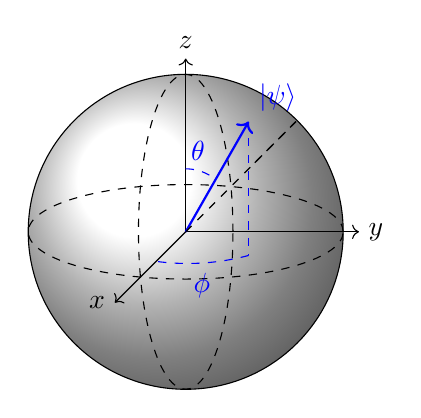
\begin{tikzpicture}
      % Draw the Bloch sphere
      \shade[ball color=white] (0,0) circle (2cm);
      \draw (0,0) circle (2cm);
      \draw[dashed] (0,0) circle (2cm and 0.6cm);
      \draw[dashed] (0,0) circle (0.6cm and 2cm);
      
      % Draw axes
      \draw[->] (0,0) -- (2.2,0) node[right] {$y$};
      \draw[->] (0,0) -- (0,2.2) node[above] {$z$};
      \draw[->] (0,0) -- (-0.9,-0.9) node[left] {$x$};
      
      % Draw state vector
      \draw[->,thick,blue] (0,0) -- (0.8,1.4) node[above right] {$|\psi\rangle$};
      
      % Draw angles
      \draw[dashed] (0,0) -- (1.4,1.4,0);
      \draw[dashed] (1.4,1.4,0) -- (1.4,1.4,1.4);
      \draw[dashed,blue] (0,0.8) arc (90:60:0.6) node[midway, above] {$\theta$};
      \draw[dashed,blue] (0.8,1.4) -- (0.8,-0.3);
      \draw[dashed,blue] (0.8,-0.3) arc (-75:-98:3) node[midway, below] {$\phi$};
  \end{tikzpicture}
  \caption{Bloch球表示}
  \label{fig:bloch_sphere}
\end{figure}

对于单个量子比特的混合态,它的密度矩阵可以表示为
\begin{equation}\label{eq:bloch_rho}
    \rho = \frac{1}{2}(I + \vec{r}\cdot\vec{\sigma}),
\end{equation}
其中$\vec{r} = (r_x, r_y, r_z)$是一个三维实向量,满足$|\vec{r}| \leq 1$,$\vec{\sigma} = (\sigma_x, \sigma_y, \sigma_z)$是Pauli矩阵,即
\begin{equation}
    \sigma_x = \begin{pmatrix} 0 & 1 \\ 1 & 0 \end{pmatrix}, \quad \sigma_y = \begin{pmatrix} 0 & -i \\ i & 0 \end{pmatrix}, \quad \sigma_z = \begin{pmatrix} 1 & 0 \\ 0 & -1 \end{pmatrix}.
\end{equation}
混合态对应的Bloch球上的点是一个三维实向量$\vec{r}$,它的长度小于等于1,即$|\vec{r}| \leq 1$。当$\norm{\vec{r}} = 1$时,即在Bloch球的表面上,对应的是一个纯态;当$\norm{\vec{r}} < 1$时,对应的点在Bloch球的内部,对应的是一个混合态。


一个由n个量子比特组成的量子系统有$2^n$个本征态,它的状态可以用长度为n的二进制串来表示,即$|x_1x_2\cdots x_n\rangle$,其中$x_i \in \{0, 1\}$。一个n量子比特的量子系统的状态可以表示为
\begin{equation}
    |\psi\rangle = \sum_{x=0}^{2^n-1} \alpha_x |x_1x_2\cdots x_n\rangle,
\end{equation}
其中$\alpha_x$是复数,满足$\sum_{x=0}^{2^n-1} |\alpha_x|^2 = 1$。
有时也会使用十进制表示,即$|x\rangle$,其中$x \in \{0, 1, \cdots, 2^n-1\}$。这样的基矢称为计算基矢(Computational Basis)。

\subsection{量子线路}
量子线路是量子计算中的一个重要概念,它描述了量子比特之间的相互作用关系。量子线路由量子门(Quantum Gate)组成,量子门是用来操作量子比特的基本单元,类似于经典计算中的逻辑门。量子门是一个幺正算符,它作用在量子比特上,改变量子比特的状态。

最简单的一类门是单比特量子门,常见的单比特量子门有Pauli门、Hadamard门、相位门、T门等。Pauli门是一组三个单比特门,分别是$X$门、$Y$门和$Z$门,它们的矩阵表示分别为
\begin{equation}
    X = \begin{pmatrix} 0 & 1 \\ 1 & 0 \end{pmatrix}, \quad Y = \begin{pmatrix} 0 & -i \\ i & 0 \end{pmatrix}, \quad Z = \begin{pmatrix} 1 & 0 \\ 0 & -1 \end{pmatrix}.
\end{equation}
Hadamard门是一个单比特门,常用于产生均匀叠加态,它常简记为H门,其矩阵表示为
\begin{equation}
    H = \frac{1}{\sqrt{2}}\begin{pmatrix} 1 & 1 \\ 1 & -1 \end{pmatrix}.
\end{equation}
上述的门矩阵表示既是幺正也是厄米的,因此既可以作为量子门,也可以作为测量算符。
另外还有两个常用的单比特门,分别是相位门(简记为$S$),还有T门,其矩阵表示分别为
\begin{equation}
    S = \begin{pmatrix} 1 & 0 \\ 0 & i \end{pmatrix}, \quad T = \begin{pmatrix} 1 & 0 \\ 0 & e^{i\pi/4} \end{pmatrix}.
\end{equation}

此外还有一类常用的含参数的单比特门,称为单比特旋转门,它们的矩阵表示为
\begin{equation}
    \begin{aligned}
        &R_X(\theta) =e^{-i\frac{\theta}{2}X} = \begin{pmatrix} \cos\frac{\theta}{2} & -i\sin\frac{\theta}{2} \\ -i\sin\frac{\theta}{2} & \cos\frac{\theta}{2} \end{pmatrix}, \\ &R_Y(\theta)=e^{-i\frac{\theta}{2}Y} = \begin{pmatrix} \cos\frac{\theta}{2} & -\sin\frac{\theta}{2} \\ \sin\frac{\theta}{2} & \cos\frac{\theta}{2} \end{pmatrix},\\ &R_Z(\theta)=e^{-i\frac{\theta}{2}Z} = \begin{pmatrix} e^{-i\theta/2} & 0 \\ 0 & e^{i\theta/2} \end{pmatrix}.
    \end{aligned}
\end{equation}
这些门可以通过旋转Bloch球来实现,从几何的角度,他们分别是将量子比特绕Bloch球的X轴、Y轴、Z轴旋转一个角度$\theta$。实际上,任意的单比特门都可以视为在Bloch球上的一个旋转操作,有如下的表示
\begin{equation}
    U = e^{i\alpha}R_n(\theta),
\end{equation}
其中$e^{i\alpha}$是一个全局相位,$R_n(\theta)$是绕Bloch球上的一个单位向量$n$旋转一个角度$\theta$,满足
\begin{equation}
    R_n(\theta) = \cos\frac{\theta}{2}I - i\sin\frac{\theta}{2}n\cdot\vec{\sigma},
\end{equation}
其中$\vec{\sigma} = (\sigma_x, \sigma_y, \sigma_z)$是Pauli矩阵向量,$n$是一个单位向量,满足$n\cdot n = 1$。
通过欧拉角分解,任意的旋转都可以表示为三个旋转门的乘积,即
\begin{equation}
    R_n(\theta) = R_Z(\beta)R_Y(\gamma)R_Z(\delta).
\end{equation}
因此,只使用两种轴的旋转门就可以实现任意的单比特门。

除了单比特门之外,还有多比特门,常见的多比特门有CNOT门。CNOT门是一个两比特门,它的矩阵表示为
\begin{equation}
    \text{CNOT} = \ketbra{0}{0}\otimes I + \ketbra{1}{1}\otimes X=\begin{pmatrix} 1 & 0 & 0 & 0 \\ 0 & 1 & 0 & 0 \\ 0 & 0 & 0 & 1 \\ 0 & 0 & 1 & 0 \end{pmatrix}.
\end{equation}

单比特旋转门的推广是多比特旋转门。为了介绍多比特旋转门,我们首先介绍Pauli word的概念。Pauli word是由Pauli算符$X$、$Y$、$Z$以及单位算符$I$进行张量积组成的一个算符,例如$XIY$、$ZZI$等。形式化地,一个长度为n的Pauli word可以表示为
\begin{equation}
    P = \bigotimes_{i=1}^n P_i,
\end{equation}
其中$P_i \in \{I, X, Y, Z\}$。
一个n-qubit的多比特旋转门是Pauli word的指数函数,即
\begin{equation}
    R_P(\theta) = e^{-i\frac{\theta}{2} P},
\end{equation}
其中$P$是一个长度为n的Pauli word,$\theta$是旋转角度。
多比特旋转门在一大类被称为变分量子算法(Variational Quantum Algorithm,VQA)中扮演着重要的角色。
多比特旋转门的实现略显复杂,但是可以通过一系列的单比特门和CNOT门来实现。

在一个量子系统中,如果能够实现任意的单比特门和CNOT门,那么这个量子系统就是通用量子计算机,可以实现任意的幺正操作。在一些特定的量子计算系统中,旋转门的实现可能会受到限制,并且旋转门的实现可能使得量子纠错变得更加困难。因此,还有一种常见的办法是使用一组固定的门集合,使得这个门集合可以实现任意的幺正操作,这样的门集合称为通用量子门集合。

常见的通用量子门集合有Clifford+T门集合。
Clifford门是一类幺正门,它们保持Pauli算符的对易关系,即对于任意的Pauli算符$P$和Clifford门$C$,有$CPC^\dagger = P'$,其中$P'$也是一个Pauli算符。Clifford门的特点是它们可以通过Hadamard门、相位门、CNOT门来构造。

将量子门按照一定的顺序组合起来,就构成了一个量子线路。量子线路是量子计算中的一个重要概念,它描述了量子比特之间的相互作用关系。量子线路由量子门组成,量子门是用来操作量子比特的基本单元,类似于经典计算中的逻辑门。量子线路的输入是一个初始的量子态,输出是一个最终的量子态。量子线路的运行过程是一个量子态在量子门作用下的演化过程,它描述了量子比特之间的相互作用关系。图~\ref{fig:quantum-circuit}展示了一个量子线路的示意图,其中包含两个被初始化为$|0\rangle$的量子比特,通过Hadamard门和CNOT门的作用,最终的量子态会被测量。

\begin{figure}[h]
    \centering
    \begin{quantikz}
        \lstick{$|0\rangle$} & \gate{H} & \ctrl{1} & \meter{} \\
        \lstick{$|0\rangle$} & \qw & \targ{} & \meter{} \\
    \end{quantikz}
    \caption{量子线路示意图}\label{fig:quantum-circuit}
\end{figure}


\subsection{量子噪声}
在实际的量子计算中,量子比特会受到噪声的影响,这会导致量子计算的结果出现误差。量子噪声是量子计算中的一个重要问题,可以通过量子信道来描述。常见的噪声分为两类,一类是保持最大混合态的噪声,称为Unital 噪声,另一类是不保持最大混合态的噪声,称为Non-unital 噪声。

由式~\ref{eq:bloch_rho},任意的单比特量子态$\rho$都可以表示为$\rho = \frac{1}{2}(I + \vec{r}\cdot\vec{\sigma})$,其中$\vec{r} = (r_x, r_y, r_z)$是一个三维实向量,满足$|\vec{r}| \leq 1$。
由于CPTP映射是线形的,任意的单比特CPTP映射$\mathcal{N}$都可以表示为
\begin{equation}
    \mathcal{N}(\rho) = \frac{1}{2}(I + \vec{r}'\cdot\vec{\sigma})= \frac{1}{2}(I + (M\vec{r}+\vec{t})\cdot\vec{\sigma}),
\end{equation}
其中$\vec{r}'$和$\vec{t}$是三维实向量,M是一个$3\times 3$的实矩阵。满足$\vec{r}'= M\vec{r}+\vec{t}$。因此,任意的单比特CPTP映射$\mathcal{N}$都可以视为是一个三维实向量$\vec{r}$的线性变换,即$\vec{r}' = M\vec{r}+\vec{t}$。

常见的一类Unital噪声是单比特Pauli噪声,它是由Pauli算符$X$、$Y$、$Z$以及单位算符$I$的概率混合而成的,即
\begin{equation}\label{eq:pauli_noise}
    \mathcal{N}(\rho) = (1-p_x-p_y-p_z)\rho + p_x X\rho X + p_y Y\rho Y + p_z Z\rho Z,
\end{equation}
其中$\rho\in \mathcal{L}(\mathbb{C}^2)$是一个单比特量子态,$X$、$Y$、$Z$是Pauli算符,$I$是单位算符,$p_x$、$p_y$、$p_z$是三个概率,满足$p_x+p_y+p_z \leq 1$。
由于$\mathcal{N}(I) = I$,$\mathcal{N}(X)=(1-2p_y-2p_z)X$,$\mathcal{N}(Y)=(1-2p_x-2p_z)Y$,$\mathcal{N}(Z)=(1-2p_x-2p_y)Z$,因此单比特Pauli噪声是Unital的。且它的作用可以表示为
\begin{equation}
    \mathcal{N}(\rho) = \frac{1}{2}(I + \vec{r}'\cdot\vec{\sigma}),
\end{equation}
其中$\vec{r}' = M\vec{r}$,$M$是一个$3\times 3$的实矩阵,满足$M = \begin{pmatrix} 1-2p_y-2p_z & 0 & 0 \\ 0 & 1-2p_x-2p_z & 0 \\ 0 & 0 & 1-2p_x-2p_y \end{pmatrix}$。

值得注意的是,任意的单比特Unital噪声都可以视为是单比特幺正操作和单比特Pauli噪声的复合,即对任意的单比特Unital CPTP映射$\mathcal{N}$,总是存在单比特幺正操作$U$和$V$,以及单比特Pauli噪声$\mathcal{N}_P$,使得
\begin{equation}
    \mathcal{N}(\rho) = V\mathcal{N}_P(U\rho U^\dagger)V^\dagger.
\end{equation}
对于Unital信道,因为$\mathcal{N}(I/2) = I/2$,所以$\vec{t} = 0$,即$\vec{r}' = M\vec{r}$。由于实矩阵$M$的奇异值分解(Singular Value Decomposition, SVD)可以表示为$M = R_1\Sigma R_2$,其中$R_1,R_2 \in SO(3)$是两个旋转矩阵,$\Sigma$是一个对角矩阵。因此,任意的Unital信道$\mathcal{N}$都可以表示为
\begin{equation}
    \mathcal{N}(\rho) = \frac{1}{2}(I + R_1\Sigma R_2\vec{r}\cdot\vec{\sigma}).
\end{equation}

由于$SU(2)\longrightarrow SO(3)$是一个双重覆盖。因此,每一个Bloch球上的旋转$R\in SO(3)$都可以由某个$U\in SU(2)$的伴随作用得到,即$R\vec{r}\cdot\vec{\sigma} = U (\vec{r}\cdot\vec{\sigma})U^\dagger$。因此,存在幺正矩阵$U$和$V$,使得
\begin{equation}
    U\rho U^\dagger = \frac{1}{2}(I + R_2\vec{r}\cdot\vec{\sigma}), \quad V\rho V^\dagger = \frac{1}{2}(I + R_1\vec{r}\cdot\vec{\sigma}).
\end{equation}

定义辅助信道$\mathcal{N'}(\rho) = V^\dagger \mathcal{N}(U^\dagger \rho U)V$,则有
\begin{equation}
    \mathcal{N'}(\rho) = \frac{1}{2}(I + \Sigma\vec{r}\cdot\vec{\sigma}).
\end{equation}
由于$\Sigma$是一个对角矩阵,因此$\mathcal{N'}$是一个单比特Pauli噪声。因此,任意的单比特Unital噪声都可以视为是单比特幺正操作和单比特Pauli噪声的复合。

除了 Unital 噪声之外,还有一类 Non-unital 噪声,Non-unital 噪声的特点是它不保持最大混合态,即$\mathcal{N}(I) \neq I$。
常见的一类 Non-unital 噪声是单比特振幅阻尼噪声(Amplitude Damping Noise),它是由振幅阻尼算符$A_0$和$A_1$构成的,即
\begin{equation}
    \mathcal{N}(\rho) = A_0\rho A_0^\dagger + A_1\rho A_1^\dagger,
\end{equation}
其中$A_0 = \begin{pmatrix} 1 & 0 \\ 0 & \sqrt{1-\gamma} \end{pmatrix}$,$A_1 = \begin{pmatrix} 0 & \sqrt{\gamma} \\ 0 & 0 \end{pmatrix}$,$\gamma$是一个强度参数,满足$0 \leq \gamma \leq 1$。


\section{张量网络图}


张量网络图记号作为一种直观的数学工具,通过几何拓扑结构将复杂的张量运算转化为可视化的图形操作。其核心思想是将张量的每个自由度(指标)表示为连接节点的“腿”(leg),张量间的缩并操作则通过腿的连接实现。

张量网络图记号的发展与量子多体物理和量子信息科学密切相关。20世纪90年代,White提出的密度矩阵重整化群(DMRG)方法首次隐式地使用了张量网络的拓扑结构。2003年,F. Verstraete等人明确提出矩阵乘积态(MPS)的图表示,标志着张量网络图记号的形式化。


在张量网络图记法中,向量作为一阶张量,可通过单个节点及其左侧延伸的线段表示:
\begin{equation}
  \ket{v}
  =
  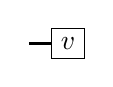
\begin{tikzpicture}[baseline=(current bounding box.center)]
    \node[draw] (s0) at (0,0) {$v$};
    \draw [thick] (-0.5,0)--(s0);
  \end{tikzpicture},
\end{equation}
其中$v=\begin{pmatrix} v_1 \\ v_2 \\ \vdots \\ v_n \end{pmatrix}$。
当给腿赋予指定的指标时,可以获得所表示向量的分量:
\begin{equation}
  \braket{i}{v}
  =v_i=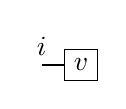
\begin{tikzpicture}
    \node[draw] (s0) at (0,0) {$v$};
    \draw [thick] (-0.5,0)--(s0);
    \node[above] at (-0.5,0) {$i$};
  \end{tikzpicture}
\end{equation}


矩阵在张量网络图中作为二阶张量,可以被表示为具有左右两侧连线的节点:
\begin{equation}
  A
  =
  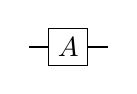
\begin{tikzpicture}[baseline=(current bounding box.center)]
    \node[draw] (s0) at (0,0) {$A$};
    \draw [thick] (-0.5,0)--(s0) (s0)--(0.5,0);
  \end{tikzpicture},
\end{equation}
其中$A=\begin{pmatrix} a_{11} & a_{12} \cdots \\ a_{21} & a_{22} \cdots \\ \vdots & \vdots \end{pmatrix}$。
矩阵的元素可通过指定连接的腿的指标获得:
\begin{equation}
  a_{ij}=
  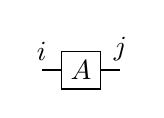
\begin{tikzpicture}[baseline=(current bounding box.center)]
    \node[draw] (s0) at (0,0) {$A$};
    \draw [thick] (-0.5,0)--(s0) (s0)--(0.5,0);
    \node[above] at (-0.5,0) {$i$};
    \node[above] at (0.5,0) {$j$};
  \end{tikzpicture}
\end{equation}


由矩阵的张量网络图表示,矩阵的转置操作可通过旋转张量对应的连接方向实现:
\begin{equation}\label{eq:tn:matrix_transpose}
  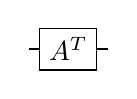
\begin{tikzpicture}[baseline=(current bounding box.center)]
    \node[draw] (s0) at (0,0) {$A^T$};
    \draw [thick] (-0.5,0)--(s0) (s0)--(0.5,0);
  \end{tikzpicture}
  =
  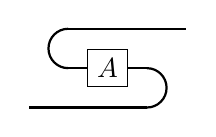
\begin{tikzpicture}[baseline=(current bounding box.center)]
    \node[draw] (s0) at (0,0) {$A$};
    \draw[thick] (-0.5,0)--(s0) (s0)--(0.5,0);
    \draw[thick] (-0.5,0.5) arc(90:270:0.25);
    \draw[thick] (0.5,-0.5) arc(-90:90:0.25);
    \draw[thick] (-0.5,0.5)--(1,0.5) (0.5,-0.5)--(-1,-0.5);
  \end{tikzpicture}
\end{equation}

对于矩阵的乘法操作,在张量网络图中是由连接相邻张量的对应边实现指标收缩来表示:
\begin{equation}\label{eq:tn:matrix_product}
  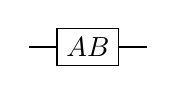
\begin{tikzpicture}[baseline=(current bounding box.center)]
    \node[draw] (s1) at (0,0) {$AB$};
    \draw [thick] (-0.75,0)--(s1) (s1)--(0.75,0);
  \end{tikzpicture}
  =
  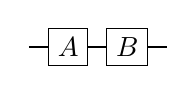
\begin{tikzpicture}[baseline=(current bounding box.center)]
    \node[draw] (s0) at (0,0) {$A$};
    \node[draw] (s1) at (0.75,0) {$B$};
    \draw [thick] (-0.5,0)--(s0) (s0)--(s1) (s1)--(1.25,0);
  \end{tikzpicture}
\end{equation}
这是因为矩阵乘法的元素表达式为
\begin{equation}
  (AB)_{ij}=\sum_k A_{ik}B_{kj}=\sum_k
  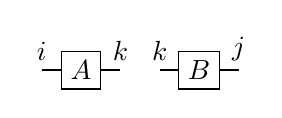
\begin{tikzpicture}[baseline=(current bounding box.center)]
    \node[draw] (s0) at (0,0) {$A$};
    \node[draw] (s1) at (1.5,0) {$B$};
    \draw [thick] (-0.5,0)--(s0) (s0)--(0.5,0) (s1)--(2,0) (s1)--(1,0);
    \node[above] at (-0.5,0) {$i$};
    \node[above] at (0.5,0) {$k$};
    \node[above] at (1,0) {$k$};
    \node[above] at (2,0) {$j$};
    \end{tikzpicture}=
    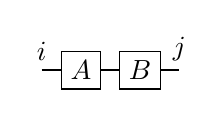
\begin{tikzpicture}[baseline=(current bounding box.center)]
        \node[draw] (s0) at (0,0) {$A$};
        \node[draw] (s1) at (0.75,0) {$B$};
        \draw [thick] (-0.5,0)--(s0) (s0)--(s1) (s1)--(1.25,0);
        \node[above] at (-0.5,0) {$i$};
        \node[above] at (1.25,0) {$j$};
    \end{tikzpicture}
\end{equation}





除了矩阵的乘法,另一种常见的张量积操作,在张量网络图中被表示为为张量的垂直堆叠:
\begin{equation}\label{eq:tn:tensor_product}
  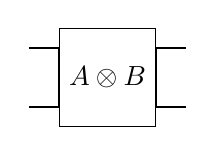
\begin{tikzpicture}[baseline=(current bounding box.center)]
    \node[draw,minimum height=1.25cm] (s1) at (0,0) {$A\otimes B$};
    \draw [thick] (-1,0.375)-|(s1.west) (-1,-0.375)-|(s1.west) (s1.east)|-(1,0.375) (s1.east)|-(1,-0.375);
  \end{tikzpicture}
  =
  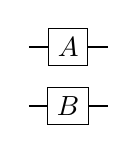
\begin{tikzpicture}[baseline=(current bounding box.center)]
    \node[draw] (s0) at (0,0) {$A$};
    \node[draw] (s1) at (0,-0.75) {$B$};
    \draw [thick] (-0.5,0)--(s0)--(0.5,0)  (-0.5,-0.75)--(s1)--(0.5,-0.75);
  \end{tikzpicture}
\end{equation}


矩阵的迹运算可以通过将张量的对应边连接并收缩来表示:
\begin{equation}\label{eq:tn:trace}
  \Tr{A}
  =
  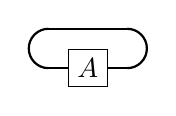
\begin{tikzpicture}[baseline=(current bounding box.center)]
    \node[draw] (s0) at (0,0) {$A$};
    \draw [thick] (-0.5,0)--(s0) (s0)--(0.5,0);
    \draw[thick] (-0.5,0.5) arc(90:270:0.25);
    \draw[thick] (0.5,0) arc(-90:90:0.25);
    \draw [thick] (-0.5,0.5)--(0.5,0.5);
  \end{tikzpicture}
\end{equation}

上述图记号通过几何拓扑直观反映了张量运算的代数结构,特别在处理高维张量收缩时,能有效降低传统指标记法的复杂性。后续章节将基于此记号体系,介绍Pauli路径积分算法的张量网络图表示。


\section{本章小结}
本章介绍了量子信息科学的基本概念,包括量子信息科学的研究背景、量子力学的基本知识、量子计算的基本概念等。介绍了表示量子系统状态的纯态、混合态、密度矩阵的概念,接着介绍了量子态的演化、量子测量的概念。最后介绍了量子计算的基本概念,包括量子比特、量子线路、量子门、量子噪声等。为了后续章节的讨论,还介绍了张量网络图的基本概念,作为一种直观的数学工具,将复杂的张量运算转化为可视化的图形操作。

在后面的章节中,我们将介绍
%#TODO



% 其他部分
\backmatter

% 参考文献
\bibliography{ref/refs}  % 参考文献使用 BibTeX 编译
% \printbibliography       % 参考文献使用 BibLaTeX 编译

% 附录
% 本科生需要将附录放到声明之后,个人简历之前
\appendix
% \input{data/appendix-survey}       % 本科生:外文资料的调研阅读报告
% \input{data/appendix-translation}  % 本科生:外文资料的书面翻译
% !TeX root = ../thuthesis-example.tex

\chapter{补充内容}

附录是与论文内容密切相关、但编入正文又影响整篇论文编排的条理和逻辑性的资料,例如某些重要的数据表格、计算程序、统计表等,是论文主体的补充内容,可根据需要设置。

附录中的图、表、数学表达式、参考文献等另行编序号,与正文分开,一律用阿拉伯数字编码,
但在数码前冠以附录的序号,例如“图~\ref{fig:appendix-figure}”,
“表~\ref{tab:appendix-table}”,“式\eqref{eq:appendix-equation}”等。


\section{插图}

% 附录中的插图示例(图~\ref{fig:appendix-figure})。

\begin{figure}
  \centering
  \includegraphics[width=0.6\linewidth]{example-image-a.pdf}
  \caption{附录中的图片示例}
  \label{fig:appendix-figure}
\end{figure}


\section{表格}

% 附录中的表格示例(表~\ref{tab:appendix-table})。

\begin{table}
  \centering
  \caption{附录中的表格示例}
  \begin{tabular}{ll}
    \toprule
    文件名          & 描述                         \\
    \midrule
    thuthesis.dtx   & 模板的源文件,包括文档和注释 \\
    thuthesis.cls   & 模板文件                     \\
    thuthesis-*.bst & BibTeX 参考文献表样式文件    \\
    thuthesis-*.bbx & BibLaTeX 参考文献表样式文件  \\
    thuthesis-*.cbx & BibLaTeX 引用样式文件        \\
    \bottomrule
  \end{tabular}
  \label{tab:appendix-table}
\end{table}


\section{数学表达式}

% 附录中的数学表达式示例(式\eqref{eq:appendix-equation})。
\begin{equation}
  \frac{1}{2 \uppi \symup{i}} \int_\gamma f = \sum_{k=1}^m n(\gamma; a_k) \mathscr{R}(f; a_k)
  \label{eq:appendix-equation}
\end{equation}


\section{文献引用}

附录中的参考文献引用

\printbibliography


% 致谢
% !TeX root = ../thuthesis-example.tex

\begin{acknowledgements}
  我谨向我的导师刘正伟表示衷心的感谢,他引领我进入了一个全新的数学研究世界。没有他持续的支持、鼓励、耐心和专业建议,这项工作无法完成。

  我还要要感谢数学中心的魏朝晖、刘子文、刘锦鹏、丁大威老师他们在同我的讨论中给予了我很多帮助。
  以及雁栖湖应用中心的程嵩老师,这项工作的一部分是在他的指导下完成的。


  最后,我要感谢我的伙伴们——陆凡、魏付川、张浩、赵子硕、李俊峰、阮钰泽、王宁烽、卢润迪、何会萱、张睿齐,以及清华的朋友们,感谢他们与我一起讨论了许多精彩的数学问题。
\end{acknowledgements}


% 声明
% 本科生开题报告不需要
\statement
% 将签字扫描后的声明文件 scan-statement.pdf 替换原始页面
% \statement[file=scan-statement.pdf]
% 本科生编译生成的声明页默认不加页脚,插入扫描版时再补上;
% 研究生编译生成时有页眉页脚,插入扫描版时不再重复。
% 也可以手动控制是否加页眉页脚
% \statement[page-style=empty]
% \statement[file=scan-statement.pdf, page-style=plain]

% 个人简历、在学期间完成的相关学术成果
% 本科生可以附个人简历,也可以不附个人简历
% !TeX root = ../thuthesis-example.tex

\begin{resume}

  \section*{个人简历}

  1997 年 11 月 11 日出生于四川省自贡市。

  2016 年 9 月考入华中科技大学数学与统计学院数学与应用数学专业,2020 年 6 月本科毕业并获得理学学士学位。

  2020 年 9 月免试进入清华大学数学科学系攻读数学博士至今。


  \section*{在学期间完成的相关学术成果}

  \subsection*{学术论文}

  \begin{achievements}
    \item Shao, Y., Wei, F., Cheng, S., \& Liu, Z. (2024). Simulating noisy variational quantum algorithms: A polynomial approach. Physical Review Letters, 133(12), 120603.
    \item Sun, W., Wei, F., Shao, Y., \& Wei, Z. (2024). Sudden death of quantum advantage in correlation generations. Science Advances, 10(47), eadr5002.
    \item Huang, Y., Shao, Y., Ren, W., Sun, J., \& Lv, D. (2023). Efficient quantum imaginary time evolution by drifting real-time evolution: An approach with low gate and measurement complexity. Journal of Chemical Theory and Computation, 19(13), 3868-3876.
    \item Shao, Y., Li, Y., Wei, F., Zhan, H., Wang, B., Wei, Z., Zhang, L., \& Liu, Z. (2024). Variational Graphical Quantum Error Correction Codes: adjustable codes from topological insights. arXiv preprint arXiv:2410.02608.
    \item Zhang, R., Shao, Y., Wei, F., Cheng, S., Wei, Z., \& Liu, Z. (2024). Clifford Perturbation Approximation for Quantum Error Mitigation. arXiv preprint arXiv:2412.09518.
  \end{achievements}

  %\subsection*{专利}

  %\begin{achievements}
    %\item 任天令, 杨轶, 朱一平, 等. 硅基铁电微声学传感器畴极化区域控制和电极连接的方法: 中国, CN1602118A[P]. 2005-03-30.
    %\item Ren T L, Yang Y, Zhu Y P, et al. Piezoelectric micro acoustic sensor based on ferroelectric materials: USA, No.11/215, 102[P]. (美国发明专利申请号.)
  %\end{achievements}

\end{resume}


% 指导教师/指导小组评语
% 本科生不需要
% !TeX root = ../thuthesis-example.tex

\begin{comments}
% \begin{comments}[name = {指导小组评语}]
% \begin{comments}[name = {Comments from Thesis Supervisor}]
% \begin{comments}[name = {Comments from Thesis Supervision Committee}]

  %论文提出了……
  暂无

\end{comments}


% 答辩委员会决议书
% 本科生不需要
% !TeX root = ../thuthesis-example.tex

\begin{resolution}
  经典模拟是研究量子算法、量子纠错、校准量子计算机的重要工具。现如今随着量子硬件的发展,传统的经典模拟方法已经逐渐逼近性能极限。在当前的时代背景下,变分量子算法因为不需要昂贵的纠错协议受到了广泛关注,但变分量子算法能否在线路噪声等实际环境下实现量子优势仍然是个困难的、被反复讨论的开放问题。

邵钰菓的博士学位论文《基于Pauli路径积分模拟量子线路》聚焦NISQ时代量子线路的经典模拟难题,提出了基于Pauli路径积分的泡利基下反向路径积分(OBPPP)算法并拓展了稀疏泡利动力学(SPD)算法,系统分析了算法的计算复杂度与误差特性,揭示了噪声对量子优势边界的临界影响。论文的主要成果如下:


1. 证明了绝大多数含噪声变分量子线路观测期望值在一定条件下的经典可模拟性。

2. 证明了在Pauli噪声率恒定或高于1/logL时,观测期望值可被多项式复杂度经典模拟;而当噪声率低于1/L时,模拟复杂度可能指数增长。

3. 通过复现IBM 127量子比特Eagle处理器的Ising模型实验,验证了该模拟算法在精度与效率上显著优于实际量子设备,并实现了噪声强度的量化评估。

研究兼具理论深度与实践价值,为量子硬件验证及噪声抑制提供了重要工具。


论文选题前沿,逻辑严谨,成果发表于《Physical Review Letters》等高水平期刊,创新性突出,理论意义与应用价值显著。答辩过程中,邵钰菓陈述清晰,表达严谨,准确回答了委员会提出的问题,展现了扎实的专业功底与独立科研能力。


经答辩委员会讨论与无记名投票,一致通过邵钰菓的博士学位论文答辩,认为这是一篇优秀的博士学位论文,建议授予邵钰菓理学博士学位。


\end{resolution}


% 本科生的综合论文训练记录表(扫描版)
% \record{file=scan-record.pdf}

\end{document}
